§ הגדרות רקורסיביות
סעיף 4ב' לחוק השבות, תש"י - 1950 קובע:
\צטט\עבה{לענין חוק זה, "יהודי" - מי שנולד לאם יהודיה או שנתגייר, והוא אינו בן
דת אחרת}.===
בבואו להגדיר את המילה "יהודי", חוק השבות משתמש בגוף ההגדרה במילה זו עצמה.
הגדרות המשתמשות במונח המוגדר כחלק מההגדרה של המונח עצמו, נקראות הגדרות
רקורסיביות. על פי ההלכה המוסלמית, מוסלמי הוא מי שנולד לאב מוסלמי או שהפך
למוסלמי באמצעות אמירת העדות, הלא היא השהאדה:
\צטט
\begin{Arabic}
  \עבה{اشهد ان لَا إِلٰهَ إِلَّا الله وان مُحَمَّدا رَسُولُ الله}
\end{Arabic}
===
(אני מעיד כי אין אלוהים לבד מאללה, וכי מוחמד הוא שליח אללה). בפני שלושה
מוסלמים. אנו רואים כי גם ההלכה המוסלמית מגדירה רקורסיבית את התשובה לשאלה "מיהו
מוסלמי?".

נאמר על קבוצה~$S$ שהיא מוגדרת באופן רקורסיבי (או בנוייה באופן רקורסיבי) אם
ההגדרה של~$S$ מבדילה בין שני סוגים של איברים: איברים אטומיים ואיברים מורכבים.
איברים מורכבים נוצרים באמצעות בנאי איברים מאיברים אטומיים ואיברים מורכבים אחרים:
\החל{ציינון}
✦ \עבה{איברים אטומיים}. בסיס הרקורסיה הוא \מונח[איבר אטומי]{איברים אטומיים},
כלומר איברים של~$S$ אשר אינם נבנים מאיברים אחרים בקבוצה. אם נביט על סעיף 4ב' של
חוק השבות כעח הגדרה רקורסיבית של קבוצת היהודים, סביר שנאמר שאברהם אבינו ושרה
אמנו הם האיברים האטומיים של הקבוצה, כלומר הם יהודים בזכות עצמם. בהסתכלות דומה
על ההלכה המוסלמית, סביר להסיק מוחמד ואולי עוד כמה מתלמידיו, הם מוסלמים מכוח
עצמם בלבד. כל שאר המוסלמים נקבעים בדרך אחרת.
✦ \עבה{בנאי איברים}. הרקורסיה עצמנה נבנית ב \מונח{בנאי איברים}, שהם כללים
המאפשרים לייצר איברים נוספים ל-$S$ מתוך איברים קיימים. איבר הנוצר על ידי בנאי
איברים, נקרא מורכב. בנאי איברים בונה איברים מורכבים של הקבוצה~$S$ מתוך איברים
אטומיים ואיברים מורכבים הקיימים בה. בהגדרה ההלכתית הרקורסיבית של קבוצות
המוסלמים יש שני בנאים:
\ספרר
✦ הבנאי שמאפשר לקבוע כי אדם מסויים הוא מוסלמי, אם אביו מוסלמי. בנאי זה הוא
בנאי \מונח{אונארי}, משום שבנאי זה מתחיל מאיבר יחיד בקבוצה, גבר שהוא מוסלמי,
ומאפשר "לבנות" איבר חדש מהאיבר הקיים.
✦ הכלל המגדיר כמוסלמי כמי שאמר את השהאדה בפני שלושה מוסלמים אחרים, הוא
בנאי \מונח{טרנארי} משום שבנאי זה מתסמך על שלושה איברים בקבוצה המוגדרת רקורסיבית
(קבוצת המוסלמים), כדי לבנות איבר חדש בקבוצה.
===

גם חוק השבות מגדיר בנאי אונארי (אמהות). החוק אמנם אינו מגדיר
במדוייק מהו גיור, אך ברור כי הגדרה מדוייקת של הגיור, תכלול רקורסיה באמצעות בנאי
איברים ובפרט, ידרש כי חברי בית הדין המחליט על הגיור יהיו יהודים בעצמם.
\סוף{ציינון}

\פסקה{הערות}
\החל{אבגוד}
✦ לעיתים נתייחס לאיברים האטומיים של קבוצה מוגדרת רקורסיבית כבנאים שהם nullary,
כלומר בנאים שאינם מקבלים ארגומנטים.
✦ גדלן של קבוצות המוגדרות רקורסיביות הוא בלתי חסום בדרך כלל, שכן תמיד ניתן
להשתמש בבנאים כדי ליצור איברים נוספים.
✦ קבוצה מוגדרת רקורסיבית יכולה להיות בעלת גודל סופי:
\ציינן
✦ אם הגדרת הקבוצה מכילה יחס שקילות, שגורים לכך שהפעלה אינסופית של בנאים, יוצרת
רק אוסף סופי של איברים שקולים.
✦ אם הבנאים אינם כאלו שתמיד ניתן להפעילם.
===
\סוף
{אבגוד}
הגדרה רקורסיבית מתאפייינת גם בתכונה נוספת:
\החל{ציינון}
✦ \עבה{שלמות ההגדרה}. הגדרה רקורסיבית של הקבוצה~$S$ כוללת תמיד בתוכה מרכיב
הדורש שאין ב~$S$ איברים אחרים מלבד האיברים האטומיים ואלו שנוצרו באמצעות בנאים.
בדרך הדרישה שבמרכיב זה של אינה נאמרת במפורש, אלא משתמעת מהניסוח. כך למשל מניסוח
חוק השבות, ברור כי ההגדרה מתכוונת לאמר שמי שאינו מקיים את התנאים המנויים בסעיף,
אינו יהודי. אך הקביעה כי כל מי שאמו אינו יהודיה ושלא התגייר איננו יהודי, אינה
מופיעה בחוק כלשונה אלא משתמעת ממנו.
\סוף{ציינון}

§§ קבוצת הפונקציות הרציונליות (הגדרה מתימטית)

נגדיר לדוגמה באופן רקורסיבי את~$ℚ₁$, קבוצת הפונקציות הרציונליות במשתנה אחד.
נסמן קבוצה זו ב~$ℚ₁$. כל איבר~$f$ בקבוצה~$ℚ₁$ הוא פונקציה חלקית מ$ℝ$, קבוצת
המספרים הממשיים אל~$ℝ$, כלומר~$f:ℝ⇸ℝ$. הכוונה במונח פונקציה חלקית היא שייתכן כי
קיים ערך מסויים~$ℝ∈x$, שעבורו ערך הפונקציה~$f)x($ אינו מוגדר. אנו נשתמש
בסימון~$⊥$ כדי לציין את הערך הלא מוגדר. ניתן לכן לכתוב~$f:ℝ→ℝ∪❴⊥❵$. בניסוח
אחר,~$ℚ₁⊆ℝ⇸ℝ$, כלומר~$ℚ₁$ היא קבוצה חלקית של קבוצת הפונצקיות החלקיות מ~$ℝ$
אל~$ℝ$.

\begin{Definition}[קבוצת הפונקציות הרציונליות]
  \label{definition:rationals}
  הקבוצה ב~$ℚ₁$, קבוצת הפונקציות הרציונליות במשתנה אחד, מוגדרת על ידי שלושת התנאים הבאים:
  \החל{ספרור}
  ✦ \עבה{איברים אטומיים של קבוצת הפונקציות הרציונליות}
  \החל{ציינון}
  ✦ הפונקציה המעתיקה כל מספר ממשי אל המספר הטבעי~$1$ נמצאת בקבוצה~$ℚ₁$, כלומר
  \begin{align}\label{eq:1}
    1∈ℚ₁
  \end{align}
  ✦ פונקצית הזהות~$I$, המעתיקה כל מספר ממשי אל עצמו נמצאת בקבוצה~$ℚ₁$, כלומר
  \begin{align}\label{eq:x}
    I∈ℚ₁
  \end{align}
  \סוף{ציינון}
  ✦ \עבה{בנאים של קבוצת הפונקציות הרציונליות}
  \החל{ציינון}
  ✦ אם הפונקציה~$f$ שייכת ל~$ℚ₁$ אזי גם הפונקציה~$-f$ שייכת לקבוצה זו
  \begin{align}\label{eq:minus}
    -f∈ℚ₁
  \end{align}
  ✦ אם הפונקציות~$f₁$ ו~$f₂$ שייכות ל~$ℚ₁$ אזי גם הסכום שלהן, המכפלה
  שלהן, והמנה שלהן שייכות ל~$ℚ₁$
  \begin{align}
    f₁+f₂ &∈ℚ₁ \label{eq:plus} ⏎
    f₁·f₂ &∈ℚ₁ \label{eq:times} ⏎
    f₁/f₂ &∈ℚ₁ \label{eq:div}
  \end{align}
  \סוף{ציינון}

  ✦ \עבה{שלמות ההגדרה: אין פונקציות רציונליות חוץ מהאטומיות ואלו שנוצרו באמצעות
  הבנאים}
 ⏎ הקבוצה~$ℚ₁$ היא הקבוצה הקטנה ביותר של פונקציות המקיימת את התנאים
  \פנה{eq:1},
  \פנה{eq:x},
  \פנה{eq:minus},
  \פנה{eq:plus},
  \פנה{eq:times}
  ו
  \פנה{eq:div}.
  \סוף{ספרור}
\end{Definition}

§§ כתיב של כללי היסק

ניסוח תמציתי ומדוייק לבנאים הוא כ\מונח{כללי היסק} כפי שהם נהוגים בתחשיב
הפסוקים. כלל היסק האומר שבכל פעם שמתקיימות ההנחות~$P₁,P₂,…,Pₙ$ ניתן להסיק את
המסקנה~$Q$ יכתב כך: \[
  \dfrac{\begin{array}{c}P₁ ⏎P₂ ⏎⋮ ⏎Pₙ\end{array}}{Q}
\] ניתן גם לכתוב את הדרישות בשורה אחת, ובלבד שהן מופרדות זו מזו, \[
  \infer Q{P₁ & P₂ &⋯& Pₙ}
\] לדוגמה, את הבנאי \פנה{eq:plus} של הקבוצה~$ℚ₁$, ניתן לכתוב ככלל היסק:
\begin{equation}\label{eq:rational:plus}
  \infer{f₁+f₂∈ℚ₁}{f₁∈ℚ₁ & f₂∈ℚ₁}
\end{equation}
בכלל היסק זה יש שתי הנחות~$P₁=f₁∈ℚ₁$ ו~$P₂=f₂∈ℚ₁$. כל אחת מההנחות צריכה להיקרא
ככמת אוניברסלי, כפי שהוא מופיע בתחשיב הפסוקים, כלומר, עבור כל בחירה של
פונקציה~$f₁$ המקיימת~$f₁∈ℚ₁$ ולכל בחירה של פונקציה~$f₂$ המקיים~$f₂∈ℚ₁$ נובעת
המסקנה~$Q=f₁+f₂∈ℚ₁$. בניסוח אחר כלל ההיסק אומר כי \[
  ∀f₁∀f₂❨f₁∈ℚ₁∧f₂∈ℚ₁→f₁+f₂∈ℚ₁❩.
\] ניתן לנסח את ארבעת הבנאים של הקבוצה~$ℚ₁$, כלומר \פנה{eq:minus},
\פנה{eq:plus},
\פנה{eq:times}
ו
\פנה{eq:div},
ככלל היסק אחד:
\begin{equation}\label{eq:rational:constructors}
  \infer{-f₁,f₁+f₂, f₁·f₂,f₁/f₂∈ℚ₁}{f₁∈ℚ₁&f₂∈ℚ₁}
\end{equation}

ניתן גם לנסח את הגדרת האיברים האטומיים של הקבוצה~$ℚ₁$, כלומר \פנה{eq:1}
ו \פנה{eq:x},
כשני כללי היסק אשר קבוצת ההנחות שלהן ריקה,
\begin{equation*}
  \begin{array}{ccc}
    \infer{I∈ℚ₁}{} & & \infer{1∈ℚ₁}{}
  \end{array}\hfill
\end{equation*}
או בקיצור, ככלל אחד,
\begin{equation}\label{eq:rational:atomic}
  \infer{1, I∈ℚ₁}{}
\end{equation}
לדוגמה,~$(I+1)/(I*I -3·I+1)$ הוא איבר ב~$ℚ₁$,
שמיייצג את הפונקציה~$f(x)=(x+1)/(x²-3x+1)$.

ניתן להשתמש במבנה ההגדרה הרקורסיבי של קבוצה בהגדרות רקורסיביות נוספות המתייחסות
לקבוצה ולאיבריה.

\begin{Definition}[ערך של פונקציה רציונלית]
  עבור פונקציה רציונלית~$f∈ℚ₁$, ועבור כל מספר ממשי~$x∈ℝ$ נגדיר את~$f(x)$
  רקורסיבית
  \begin{equation}\label{eq:value}
    \begin{array}{cc}
      1(x)=1 & I(x)=x ⏎ ⏎
      \infer{-f(x)=-x₁}{f(x)=x₁} & \infer{(f₁+f₂)(x)=x₁+x₂}{f₁(x)=x₁ & f₂(x)=x₂} ⏎ ⏎
      \infer{(f₁·f₂)(x)=x₁·x₂}{f₁(x)=x₁ & f₂(x)=x₂} &
      \infer{(f₁/f₂)(x)=x₁/x₂}{f₁(x)=x₁ & f₂(x)=x₂}
    \end{array}
  \end{equation}
\end{Definition}

§§ אינדוקצית מבנה
הגדרות רקורסיביות מאפשרות לנו להוכיח טענות באינדוקציה הידועה בשם אינדוקצית
מבנה. באינדוקציה כזו, אנו מוכיחים ראשית כי הטענה נכונה עבור כל האיברים האטומיים
של קבוצה. בצעד האינדוקציה נעבור על כל בנאי האיברים: לגבי כל בנאי נניח שהטענה
נכונה לגבי כל האיברים עליהם פועל, ונוכיח כי הטענה נכונה גם עבור האיבר אשר אותו
יצר הבנאי. ניתן גם להסתכל על הוכחות באינדוקצית מבנה כאינדוקציה על מספר
ההפעלות~$n$ של בנאים לשם יצירת~$f$.

נוכיח לדוגמה את הטענה הפשוטה הבאה עבור ההגדרה הרקורסיבית של הקבוצה~$ℚ₁$
(\פנה{definition:rationals}) וההגדרה של ערך הפונקציה מעל \פנה{eq:value}.

\begin{Claim}
  עבור כל מספר רציונלי~$q∈ℚ$, ועבור כל פונקציה רציונלית~$f∈ℚ₁$, מתקיים כי
  \begin{equation}\label{eq:Q}
    f(q)∈ℚ∪❴⊥❵
  \end{equation}
  כלומר~$f(q)$ אינו מוגדר, או שהוא מספר רציונלי.
\end{Claim}

\begin{proof}
  \mbox{}
  \תאר
  ✦[בסיס האינדוקציה] אם~$n=0$ אז~$f$ הוא איבר אטומי של~$ℚ₁$, ואז~%~$f=1$ או~%
  $f=I$ וברור שאם~$q$ רציונלי, אז גם~$f(q)∈❴1,q❵$. ולכן \פנה{eq:Q}
  מתקיימת עבור~$n=$0.
  ✦ [צעד האינדוקציה] נניח שהטענה \פנה{eq:Q} מתקיימת עבור כל~$n'$, כאשר~$n'<n$
  ונוכיח אותה עבור~$n$.

  נסתכל על איבר~$f∈ℚ₁$ אשר נוצר מהפעלה של~$n$ בנאים, ונניח ש~$n>0$ כלומר~$f$
  נוצר על ידי הפעלה של בנאי. בנאי זה הוא אחד מארבעת הבנאים \פנה{eq:minus},
  \פנה{eq:plus}, \פנה{eq:times}, או \פנה{eq:div}.
  מכאן, \[
    f(q)∈❴-q₁,q₁+q₂,q₁·q₂,q₁/q₂❵.
\] כיוון שמספר הפעלות הבנאים לשם יצירת הפונקציות~$f₁$ ו~$f₂$ קטן ממש מ-$n$ הנחת האינדוקציה מתקיימת לגביהן, ולכן, על גם~$q₁$ וגם~$q₂$ חייבים להיות רציונליים אם הם מוגדרים,
  ולכן גם~$f(q)$, אם הוא מוגדר, חייב להיות מספר רציונלי.
===
\end{proof}

§§ שימוש בהגדרות רקורסיביות באיפיון של שפת תכנות
הגדרות רקורסיביות משמשות לעיתים קרובות באיפיון של שפות תכנות.
הנה כמה דוגמאות.

\begin{Example}[ביטויים בשפות תכנות]
  בשפות תכנות כמו פסקל קבוצת הביטויים האריתמטיים אותה ניתן לכתוב בתכניות בשפה מוגדרת רקורסיבית:
  \אבגד
  ✦ הביטויים
  האטומיים כוללים מספרים, כגון המספר השלם
  \קד{21} והמספר הממשי
  \קד{13.4}
  והפניות למשתנים, כגון \קד{x}.
  ✦בנאי הביטויים הם האופרטורים וסימני הפונקציה:
  אופרטורים אונאריים כגון סימן המינוס החד מקומי (\קד{-$·$}) הם בנאי ביטויים אונאריים.
  אופרטורים בינאריים, כגון החיבור (\קד{$·$+$·$}) והכפל (\קד{$·$*$·$}) הם בנאי
  ביטויים בינאריים. כל פונקציה של פסקל, בין אם היא מוגדרת בשפה ובין אם היא הוגדרה על ידי המתכנת, גם היא בנאי ביטויים. פונקציה המקבלת~$n$ ארגומנטים היא בנאי ביטויים~$n$ מקומי.
===
  לדוגמה, בשפת \פסקל הביטוי
  \begin{PASCAL}
(-12+sin(13.4)) * x
\end{PASCAL}
  הוא ביטוי מורכב המכיל בתוכו שלושה ביטויים אטומיים
  \קד{12}, \קד{13.4} ו-\קד{x}. בביטוי מופיע בנאי בינארי אחד (\קד{$·$*$·$}), ושלושה בנאים אונאריים: סימן המינוס החד מקומי (\קד{-$·$}), הפונקציה החד מקומית \קד{sin($·$)}, וגם בנאי אונארי נוסף המאפשר לעטוף ביטוי בסוגרים. על פי בנאי זה, אם~$E$ הוא ביטוי אזי גם
  \קד{($E$)} הוא ביטוי, ועל כן, כיוון ש \קד{-12+sin(13.4)} הוא ביטוי
  אזי גם \קד{(-12+sin(13.4))} הוא ביטוי.
\end{Example}

לבד מביטויים, תכניות גם מכילות פקודות אשר ביצוען מביא לשינוי של מצב התכנית. גם קבוצת הפקודות מוגדרת בדרך כלל רקורסיבית.

\begin{Example}[פקודות בשפת פסקל]
  לדוגמה בפסקל ישנן פקודות אטומיות מארבעה סוגים:
  ⌘החל{ספרור}
    ✦ \עבה{קריאה לפרוצדורה}. זוהי פקודה כגון
    \begin{PASCAL}
WriteLn('Hello, World')
\end{PASCAL}
    אשר קוראת לפרוצדורה המוגדרת בשפה, או פרוצדורה המוגדרת על ידי המתכנת, כמו
    \begin{PASCAL}
ComputeSolution(1,5,6,x)
\end{PASCAL}
    ✦ \עבה{פקודת השמה}. זוהי פקודה כגון
    \begin{PASCAL}
x:=(-12+sin(13.4))*x
\end{PASCAL}
    אשר בה מחושב ערך ומוצב למשתנה. נשים לב לכך שעל אף שהפקודה
    היא פקודה אטומית, הפקודה מכילה בתוכה ביטוי מורכב.
    ✦ \עבה{פקודת קפיצה}. זוהי פקודה כגון
    \begin{PASCAL}
goto 999
\end{PASCAL}
    אשר בה בקרת הזרימה מועברת למקום אחר בתכנית. בדוגמה שלנו, הפקודה המסומנת בתגית 999.

    ✦ \עבה{הפקודה הריקה}. זוהי פקודה שאינה עושה דבר. אין צורך לכתוב דבר כדי להשתמש בפקודה זו, והיא משמשת בעיקר לצורך בניית פקודות מורכבות
  ⌘גמר{ספרור}
  בשפת פסקל יש גם בנאי פקודות. החשובים ביותר הם אלו:
  ⌘החל{ספרור}
    ✦ \עבה{בנאי הבלוק}. סדרה של פקודות המופרדות על ידי סימן הנקודה ופסיק (\קד{;})
    והעטופה במילים \מש{begin} ו\מש{end} גם היא פקודה. בנאי הבלוק הוא בנאי רב מקומי, שיכול לקבל מספר כלשהו של פקודות, מורכבות או אטומיות, ולבנות מהם פקודה אחת. זו לדוגמה פקודה מורכבת הנוצרת על ידי בנאי
    הבלוק משתי פקודות אטומיות.
    \begin{PASCAL}
begin
  a:=b;
  goto 999
end
\end{PASCAL}
    נשים לב לכך שסימן הנקודה ופסיק (\קד{;}) מפריד בין פקודות ואינו חלק מהפקודה.
    לכן,
    \begin{PASCAL}
begin
  a:=b;
  goto 999;
end
\end{PASCAL}
    היא פקודה מורכבת הנוצרת משלוש פקודות אטומיות, שהאחרונה בהן ריקה. בנאי הבלוק הוא גם nullary, וגם
    \begin{PASCAL}
begin
end
\end{PASCAL}
    היא פקודה.
    ✦ \עבה{בנאי לולאת ה-\קד{while}}. בנאי לולאת ה-\קד{while} הוא בנאי אונארי: אם~$C$ היא פקודה ו-$E$ הוא ביטוי בוליאני, אזי גם לולאת ה\קד{while}
    \begin{PASCAL}
while ⌘$E$⌘ do ⌘$C$⌘
\end{PASCAL}
    היא פקודה. על פי בנאי זה,
    \begin{PASCAL}
while x > sin(x) do x :=sin(x)
\end{PASCAL}
    ✦ \עבה{בנאי התנאי חלקי}. גם בנאי התנאי חלקי הוא בנאי אונארי. לפי בנאי זה, אם~$C$ היא פקודה ו-$E$ הוא ביטוי בוליאני, אזי גם פקודת התנאי החלקי היא פקודה:
    \begin{PASCAL}
if ⌘$E$⌘ then ⌘$C$⌘
\end{PASCAL}
    ✦ \עבה{בנאי התנאי המלא}. אם~$C₁$ ו~$C₂$ הן פקודות ו-$E$ הוא ביטוי בוליאני, אזי
    גם פקודת התנאי המלא היא פקודה:
    \begin{PASCAL}
if ⌘$E$⌘ then ⌘$C₁$⌘ else ⌘$C₂$⌘
\end{PASCAL}
    היא פקודה.
  ⌘גמר{ספרור}
\end{Example}

§ אלפאבית, מילים, ושפות פורמליות
אלפאבית הוא קבוצה, בדרך כלל סופית, של אותיות. לדוגמה הקבוצה~$❴⌘a,⌘b,⌘c❵$ הינה
אלפאבית המכיל שלוש אותיות,~$⌘a$,~$⌘b$ ו~$⌘c$. לאותיות האלפאבית אין משמעות מלבד
העובדה שכולן שונות זו מזו. כד להבדיל בין אות שאינה מציינת דבר, ובין אות המציינת
ערך, נשתמש בגופן שונה. הכתיב~$⌘a$ מכוון אל האות הראשונה באלפאבית הלטיני, ולא
למה שאות זו מציינת, ואילו הכתיב~$a$ יתייחס למה שהאות הראשונה מציינת, למשל
במשוואה הריבועית \[
  a x²+bx+c=0
\] האות~$a$ מציינת את המקדם של~$x²$ במשוואה.

\begin{Example}
  האלפאבית~$Σ_C$ המשמש לכתיבת תכניות בשפת~\CPL מכיל את 95 תווים הנחלקות, לשם נוחות בלבד, לקבוצות הבאות:
  \begin{equation}\label{alpahet:C}
  Σ_C=
  Σ_{\text{upper}}∪
  Σ_{\text{lower}}∪
  Σ_{\text{digit}}∪
  Σ_{text{special}}∪
  Σ_{\text{space}}
  .
\end{equation}
\החל{ספרור}
✦ \עבה{26 אותיות אנגליות גדולות} \[
Σ_{\text{upper}}=❴⌘A,⌘B,⌘C,⌘D,⌘E,⌘F,⌘G,⌘H,⌘I,⌘J,⌘K,⌘L,⌘M,⌘N,⌘O,⌘P,⌘Q,⌘R,⌘S,⌘T,⌘U,⌘V,⌘W,⌘X,⌘Y,⌘Z❵.
\] ✦ \עבה{26 אותיות אנגליות קטנות} \[
  Σ_{\text{lower}}=
❴⌘a,⌘b,⌘c,⌘d,⌘e,⌘f,⌘g,⌘h,⌘i,⌘j,⌘k,⌘l,⌘m,⌘n,⌘o,⌘p,⌘q,⌘r,⌘s,⌘t,⌘u,⌘v,⌘w,⌘x,⌘y,⌘z❵
.
\] ✦ \עבה{10 ספרות} \[
Σ_{\text{digit}}=❴⌘0,⌘1,⌘2,⌘3,⌘4,⌘5,⌘6,⌘7,⌘8,⌘9❵.
\] ✦ \עבה{29 אותיות מיוחדות} \[
  Σ_{\text{special}}=
  Σ_{\text{punctuation}}∪
  Σ_{\text{wrapping}}∪
  Σ_{\text{arithmetic}}∪
  Σ_{\text{other}}∪
  Σ_{\text{space}}
  .
\] המתחלקות באופן הבא:
\החל{ספרור}
✦ \עבה{8 אותיות פיסוק} \[
    Σ_{\text{punctuation}}=❰⌘., ⌘,, ⌘?, ⌘!, ⌘:, ⌘;, ⌘', ⌘"❱.
\] ✦ \עבה{6 אותיות אריתמטיות} \[
  Σ_{\text{arithmetic}}=❰⌘+, ⌘*, ⌘/, ⌘-, ⌘<, ⌘>❱.
\] ✦ \עבה{6 אותיות סוגריים} \[
    Σ_{\text{wrapping}}=❰⌘(, ⌘), ⌘[ ⌘], ⌘❴, ⌘❵,❱.
\] ✦ \עבה{9 אותיות אחרות} \[
    Σ_{\text{other}}=❰⌘&,⌘\textbackslash, ⌘\textasciicircum, ⌘\_, ⌘|, ⌘∿, ⌘\$,
  ⌘\%, ⌘#,❱.
\] \סוף{ספרור}
✦ \עבה{6 אותיות רווח} \[
    Σ_{\text{space}}=❰\text{space},\text{tab},
  \text{horizontal tab}, \text{new line},
\text{vertical tab}, \text{form feed}❱.
\] היצוג הגרפי של אותיות אלו הינו בלתי נראה, ולכן
כתבנו כאן את שמות האותיות, ולא את היצוג הגרפי שלהן.
\סוף{ספרור}
\end{Example}

מילה מעל האלפאבית היא סדרה סופית של אותיות מתוך האלפאבית. למשל,~$⌘{caba}$ היא
מילה בת ארבע אותיות מעל האלפאבית~$❴⌘a,⌘b,⌘c❵$. בהינתן אלפאבית~$Σ$, נסמן
ב~$Σ^*$ את הקבוצה האינסופית המכילה את כל המילים באורך סופי מעל~$Σ$, לרבות
המילה הריקה, אותה בדרך כלל מסמנים ב~$ε$. בדוגמה שלנו
\begin{equation}
  ❴⌘a,⌘b,⌘c❵^*=❴ε,⌘a,⌘b,⌘c,⌘{aa},⌘{ab},⌘{ac},⌘{ba},⌘{bb},⌘{bc},⌘{ca},⌘{cb},⌘{cc},⌘{aaa},⌘{aab},…❵
\end{equation}

ניתן גם להגדיר את~$Σ^*$ רקורסיבית. בהגדרה זו, יהיה איבר אטומי אחד, המילה
הריקה~$ε$, ובנאי אונארי שמאפשר להאריך כל מילה ב~$Σ^*$ באות מתוך~$Σ$:

\begin{Definition}[המילים מעל אלפאבית]
  בהנתן אלפאבית~$Σ$ אזי~$Σ^*$, קבוצת ה\עבה{המילים הפורמליות} מעל~$Σ$, מוגדרת
  באמצעות הבנאי הנולארי (המגדיר איבר אטומי אחד ויחיד)
  \begin{equation}
    \infer{ε∈Σ^*}{}
  \end{equation}
  והבנאי האונארי:
  \begin{equation}
    \infer{wσ∈Σ^*}{w∈Σ^* &σ∈Σ}
  \end{equation}
\end{Definition}

בהסתמך על הגדרה רקורסיבית זו, נגדיר רקורסיבית את~$|w|$, מספר התווים במילה~$w$:
\begin{Definition}[אורך מילה]\label{definition:length}
  עבור~$w∈Σ^*$
  \begin{equation}
    |w|=\begin{cases}
      |w'|+1 & w=w'σ ⏎
      0 & w=ε. ⏎
    \end{cases}
  \end{equation}
\end{Definition}

כך נקבל ש~$|ε=1|$,~$|⌘a|=1$,~$|⌘{caa}|=3$.

שפה פורמלית~$L$ מעל~$Σ$ היא אוסף של מילים הלקוחות מ~$Σ^*$, כלומר~$L⊆Σ^*$.

\begin{Example}[שפת התכנות~\CPL כשפה פורמלית]
  שפת התכנות~\CPL מגדירה שפה פורמלית~$L₀$ מעל האלפאבית
  $Σ_C$ \פנה{eq:alphabet:C}:
  נאמר על מילה~$w$
  (כאשר~$w∈Σ_C^*$),
  כי היא שייכת לשפה~$L₀$
  אם ורק אם~$w$ היא תכנית חוקית בשפת~\CPL.
\end{Example}
    למעשה, כל שפת תכנות תגידה שפה פורמלית, המוגדרת על ידי כל התכניות החוקיות בשפה.

§§ קבוצת הפונקציות הרציונליות כשפה פורמלית

נגדיר לדוגמה באופן רקורסיבי את השפה הפורמלית~$L₁$ שכל מילה בה יכולה להתפרש
כאיבר ב~$ℚ₁$.
\אבגד
✦ המילים האטומיות בשפה זו יהיו האותיות הבודדות 1⌘ ו I⌘. כשנגדיר פונקציה המעניקה
משמעות לכל מילה בשפה הפורמלית~$L₁$, את שתי האותיות 1⌘ ו I⌘ כפונקצית היחידה
וכפונקצית הזהות.
✦ בנוסף נשתמש באותיות ⌘/ ⌘* ⌘+⌘-. כשפה פורמלית, לא תהיינה לאותיות אלו משמעות,
אך כשנגדיר פונקציה המעניקה משמעות לכל מילה בשפה הפורמלית, פונקציה זו תפרש ארבע
אותיות אלו כאופרטורים האריתמטיים.
✦ על שש אותיות אלו נוסיף גם את האותיות ⌘(ו ⌘) וזאת בכדי להבטיח שתהיה רק דרך אחת
לתת משמעות למילה בשפה הפורמלית~$L₁$.===

\begin{Definition}[השפה הפורמלית של הפונקציות הרציונליות]
  \label{definition:L1}
  השפה~$L₁$, היא שפה פורמלית מעל האלפאבית
  \begin{equation}\label{eq:Q:alphabet}
    ❴⌘1, ⌘I, ⌘(, ⌘), ⌘/, ⌘*, ⌘+, ⌘-❵
  \end{equation}
  המוגדרת על ידי שני איברים אטומיים
  \begin{align}
     & \infer{⌘1∈ℚ₁}{} ⏎
     & \infer{⌘I∈ℚ₁}{}
  \end{align}
  ועל ידי ארבעה בנאים:
  \begin{align}
     & \infer{⌘)⌘-w⌘(∈L₁}{w∈L}⏎
     & \infer{⌘)w₁⌘+w₂⌘(∈L₁}{w₁∈ℚ₁ & w₂∈L₁}⏎
     & \infer{⌘)w₁⌘*w₂⌘(∈L₁}{w₁∈L₁ & w₂∈L₁}⏎
     & \infer{⌘)w₁⌘/w₂⌘(∈L₁}{w₁∈L₁ & w₂∈L₁}\label{eq:Q:constructors}
  \end{align}
\end{Definition}
כדאי לשים לב להבדלים בין הגדרה זו ובין ההגדרה הקודמת של הקבוצה~$ℚ₁$
(\פנה{definition:rational}). הגדרה
הנוכחית אינה מניחה ידע במתימטיקה או בפעולות החשבון. איבר של הקבוצה היא סדרה ללא
משמעות אותיות הלקוחה מהאלפאבית \פנה{eq:Q:alphabet}.

עוד נשים לב כי

§§ ההיררכיה של חומסקי
הנה עוד כמה שפות פורמליות מעל האלפאבית~$❴⌘a,⌘b,⌘c❵$:

\ציינן
✦ השפה~$L₂$ המוגדרת את כל המילים שהן פלינדרום, כלומר, מילים כמו~$⌘{aba}$ אשר
שלא תשתננה גם אם תיקראנה מסופן.
✦ השפה~$L₃$ הכוללת את כל המילים המתחילות ב~$⌘a$ ונגמרות ב~$⌘c$.
✦ השפה~$L₄$ שפת המילים שהאותיות שלהן מופיעות בסדר אלפאביתי לא יורד.
✦ השפה~$L₅$ שפת המילים שמכילות חמש אותיות או יותר.
✦ השפה~$L₆$ שפת המילים שכל אותיותיהן שונות.
===

שפה פורמלית יכולה להיות סופית או אינסופית. שפה סופית ניתנת תמיד לתאור מדוייק
באמצעות מניית כל המילים בשפה. ברשימה לעיל כל השפות הן שפות אינסופיות מלבד השפה
האחרונה~$L₆$ המכילה בדיוק 13 מילים
\begin{equation}\label{eq:L6}
  L₆=❴ε,⌘a,⌘b,⌘c,⌘{ab},⌘{ac},⌘{ba},⌘{bc},⌘{ca},⌘{cb},⌘{abc},⌘{acb},⌘{bac},⌘{bca},⌘{cab},⌘{cba}❵.
\end{equation}
את השפה האינסופית~$L₅$ ניתן להגדיר תוך שימוש בהגרה \פנה{definition:length}
\begin{equation}\label{eq:L5}
  L₅=❴w \,|\, w∈Σ^*, |w|≥5❵.
\end{equation}

כל ההגדרות המדוייקות של השפות הפורמליות
$L₆$ \cref{eq:L6},
$L₅$ \cref{eq:L5},
ו-~$L₁$
(\cref{definition:L1})
היו שונות זו מזו,
וכולן היו, במובן מסויים אד-הוק.
כלומר, עבור כל השפ בחנו בשיטת הגדרה
המתאימה לה.

אנו מתעניינים במנגנונים כלליים להגדרת שפות פורמליות.
ארבעת המנגנונים העיקריים הם:
\begin{enumerate}
  \item \עבה{ביטויים רגולריים} (\LR{regular expressions})
    אותם נכיר ב \cref{section:regular}.
  \item \עבה{שפות חסרות הקקשר רגולריים} (\LR{regular expressions})
    אותם נכיר ב \cref{section:regular}.

קבוצת כל השפות מעל~$Σ$ היא לכן קבוצת כל הקבוצות החלקיות של~$Σ^*$, כלומר קבוצת
החזקה של~$Σ^*$, אותה נסמן ב-$𝒫Σ^*$. נסמן ב-\textbf{Finite} את קבוצת כל השפות
הסופיות. ראינו כבר כי \[
  L₆∈\text{\textbf{Finite}}.
\] נסמן ב-\textbf{Regular} את קבוצת כל השפות הפורמליות הרגולריות, כלומר
השפות שאותן ניתן לתאר באמצעות ביטוי רגולרי.
כאמור \[
  L₃,L₄,L₅∈\text{\textbf{Regular}}.
\] נסמן ב-\textbf{CFG} את קבוצת כל השפות הפורמליות חסרות ההקשר, כלומר אותן השפות
שאותן ניתן לתאר באמצעות דקדוק חסר הקשר.
כאמור \[
  L₁,L₂∈\text{\textbf{CFG}}.
\] מתברר כי:
\begin{equation*}
  \text{\bfseries Finite}⊊\text{\bfseries Regular}⊊\text{\bfseries CFG}⊊
  \text{\bfseries CSG}⊊𝒫Σ^*.
\end{equation*}
כלומר, ניתן לתאר את כל השפות הסופיות באמצעות ביטוויים רגולריים, אך לא כל השפות
שאפשר לתאר אותן בביטוי רגולרי הן סופיות. בנוסף, כל שפה שאפשר לתאר באמצעות
ביטויים רגולריים, ניתן גם לתאר באמצעות דקדוק חסר הקשר, אך יש שפות שניתן לתאר
באמצעות דקדוקים חסרי הקשר, ושאי אפשר לתאר באמצעות ביטויים רגולריים. יתירה מכך,
ישנן שפות אותן לא ניתן לתאר באמצעות דקדוקים חסרי הקשר.

עוד מתברר כי
\begin{equation}
  L₀∉\text{\bfseries CFG}
\end{equation}
כלומר, לא ניתן לתאר את שפת~\CPL באמצעות דקדוקיחם חסרי הקשר.

    ביטויים רגולריים, אותם נכיר ב\cref{section:regular} מאפשרים להגדיר שפות
    פשוטות כגון~$L₄$ ו~$L₅$.
  \item \עבה{דקדוקים חסרי הקשר רגולריים}
  \item \עבה{דקדוקים תלויי הקשר}
  \item \עבה{הגדרה באמצעות תכנית}
\end{enumerate}

הגדרה פורמלית של השפות~$L₁$ ו~$L₂$
דורשת שימוש במנגנון שנכיר בהמשך, דקדוקים חסרי הקשר (\LR{context free
  grammars}). הגדרה מדיוקת של השפות~$L₃$ ו~$L₄$
דורשת שימוש במנגנון אחר, ביטויים רגולריים
§ עצים וביטויים
§§ עצים
נגדיר גם את~$T(Σ)$, קבוצת העצים שבכל צומת שלהם ישנו איבר של~$Σ$.
עץ כזה יכול להיות עץ אטומי, ואז העץ מצטמצם לכדי עלה בודד, שחייב להכיל איבר
של~$Σ$. עץ ב~$T(Σ)$ יכול להיות גם עץ מורכב, ובמקרה זה הוא מכיל מצומת פנימית
המכילה איבר של~$Σ$ ומספר כלשהו של בנים שכולם עצים ב~$T(S)$. למעשה, עץ אטומי הוא
עץ מורכב שיש לו אפס בנים.

פורמלית, קבוצת העצים~$T(Σ)$ היא מילה בשפה מעל האלפאבית המכיל את Σ ושלושה סימנים
נוספים: סימן הפסיק וסימני הסוגריים העגולים.
\begin{Definition}[עצים מעל אלפאבית]
  בהנתן אלפאבית~$Σ$
  אזי,~$T(Σ)$,
  קבוצת העצים מעל~$Σ$
  מוגדרת באמצעות הבנאי ה-$n$ מקומי,
  \begin{equation}
    \infer{σ(τ₁,⋯,τₙ)∈T(Σ)}{σ∈Σ & n≥0 &τ₁∈T(Σ) &⋯&τₙ∈T(Σ) }
  \end{equation}
  עבור כל~$n≥0$.
\end{Definition}
כמה איברים של קבוצת העצים מעל האלפאבית בן שלוש האותיות שלנו הם \[
  a, b, c,
  a(b,c), a(b(a),a(a,b,c)).
\] ויזואלית, ששת העצים הללו נראים כך
\begin{figure}
  \centering
  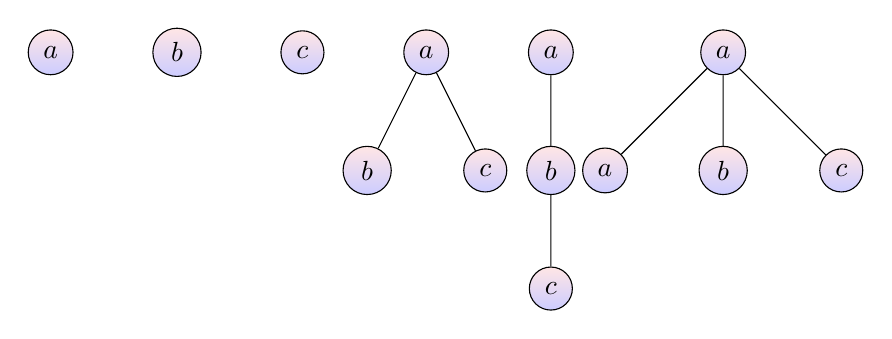
\begin{tikzpicture}[every node/.style={shape=circle, draw, align=center,
          top color=red!10, bottom color=blue!20}]
    \usetikzlibrary{trees,chains}
    \begin{scope}[start chain=growing right]
      \node[on chain]{$a$};
      \node[on chain]{$b$};
      \node[on chain]{$c$};
      \node[on chain]{$a$} child{node{$b$}} child{node{$c$}};
      \node[on chain]{$a$} child{node{$b$} child{node{$c$}}};
      \node[on chain,xshift=4ex]{$a$}child {node{$a$}} child {node{$b$}} child{node{$c$}};
    \end{scope}
  \end{tikzpicture}
\end{figure}

§ חתימות וביטויים פורמליים

אנו רואים באיור שמספר הבנים של צומת המכיל את האות~$a$ אינו קבוע. בחלק מהעצים
לצומת זה אין בנים כלל, ואילו בעצים אחרים יש לצומת זה בן אחד, שני בנים, ואף
שלושה. כדי להגדיר עצים שבהם לכל צומת מסוג מסויים יש תמיד מספר בנים, נזדקק למושג
החתימה.

\begin{Definition}[חתימה] חתימה~$Γ$, הינה אלפאבית, (בדרך כלל סופי)
  עליו מוגדרת פונקצית ערכיות~$\arity$ המתאימה לכל אות~$γ∈Γ$ מספר שלם אי
  שלילי,~$\arity:Σ→ℕ⁺$.
\end{Definition}
עבור חתימה~$Γ$, נסמן ב~$Γₙ$
את תת הקבוצה של איברי~$Γ$
שה-$\arity$ שלהם הוא~$n$
\begin{equation*}
  Γₙ=❴γ∈Γ\,|\,\arity(γ)=n❵.
\end{equation*}

ביטויים פורמליים מעל חתימה דומים לעצים מעל אלפאבית, בצירוף המגבלה שלצומת המסומנת באות~$n_γ∈Γ$,
יש בדיוק~$\arity(γ)$ בנים. פורמלית,

\begin{Definition}[ביטויים פורמליים מעל חתימה]
  בהנתן חתימה~$Γ$
  אזי,~$E(Γ)$,
  קבוצת הביטויים הפורמליים מעל~$Γ$
  מוגדרת באמצעות הבנאי ה-$n$ מקומי,

  \begin{equation*}
    \infer{σ(τ₁,⋯,τₙ)∈T(Γ)}{σ∈Σ & n≥0 &γ∈Γₙ&τ₁∈T(Γ) &⋯&τₙ∈T(Γ) }
  \end{equation*}
\end{Definition}
\פסקה{דוגמה: ביטויים סימבוליים כביטויים פורמליים}
בהינתן אלפאבית~$Σ$, נבנה ממנו חתימה~$Γ$ באופן הבא:
\begin{align*}
   & Γ=Γ₀∪Γ₂ ⏎
   & Γ₀=Σ ⏎
   & Γ₂=❴.❵
\end{align*}
קל לראות שהביטויים הפורמליים ב-$E(Γ)$ הם בדיוק בעלי אותו מבנה כמו הביטויים
הסימבוליים בקבוצה~$S)Σ$.

\פסקה{דוגמה: ביטויים חשבוניים}
נסתכל למשל על החתימה הבאה
\begin{equation}
  \begin{split}
  % & Γ=Γ₀∪Γ₁∪Γ₂ ⏎
  % & Γ₀=❰⌘0,⌘1,⌘2,⌘3,⌘4,⌘5,⌘6,⌘7,⌘8,⌘9❱^*⏎
  % &\quad=❴⌘0,⌘1,⌘2,…,⌘10,⌘11,…,⌘{100},⌘{101},…,⌘{1000},⌘{1001},…❵ ⏎
  % & Γ₁=❴⌘-,⌘!,⌘{$√$}❵ ⏎
    & Γ₂=❴⌘+,⌘*,⌘/❵
  \end{split}
\end{equation}
חתימה זז היא חתימה אינסופית בגודלה, שבה ה-arity של הסימנים~$⌘+$,~$⌘*$ ו~$⌘/$
הוא 2, ה-arity של הסימנים ⌘!,
ו~$⌘-$ הוא 1, וה-arity של קבוצת המספרים
הטבעיים הוא 0. קבוצת הביטויים מעל חתימה זו היא לא אחרת מאשר קבוצת הביטויים
החשבוניים הבנויים ממספרים הטבעיים, האופרטורים הבינאריים של חיבור, כפל וחילוק,
והאופטורים האונאריים של השלילה, העצרת, והוצאת השורש. כמה ביטויים בקבוצה זו
מודגמים באיור הבא:

\begin{figure}
  \centering
  \begin{tikzpicture}[every node/.style={shape=circle,
          draw, align=center,
          top color=red!10, bottom color=blue!20}]
    \begin{scope}[yshift=-10ex,start chain=growing right,minimum size=2em]
      \node[on chain,circle,draw]{⌘1};
      \node[on chain,circle,draw]{⌘0};
      \node[on chain,circle,draw]{⌘!} child {node {⌘3}};
      \node[on chain,circle,draw]{⌘!} child {node{⌘*} child{node{⌘a}} child{node{⌘-} child{node{42}}}};
% \node[on chain,circle,draw,xshift=5ex]{⌘√{}}
      child {node{⌘/}
          child {node{5}}
          child {node{3}}
        }
      ;
    \end{scope}
  \end{tikzpicture}
\end{figure}

נשים לב שההגדרה במובן זה שהיא קובעת את מבנה העצים, ולא את המשמעות שלהם. אין שום
דבר בהגדרה הנותן משמעות של חיבור לסימן ה-+. ההגדרה גם אינה מעניקה משמעות לקבוצת
המספרים הטבעיים. לדידה של ההגדרה, מספר טבעי הוא סדרת ספרות
נטולת משמעות.

§ ביטויים רגולריים

ביטויים רגולריים הם מכשיר חשוב להגדרת שפות פורמליות מעל אלפאבית נתון. ביטויים
רגולריים דומים במבנה שלהם לביטויים חשבוניים: הם עצים, אשר בצמתים פנימיים נמצא
אופרטורים בעלי arity ידוע, כאשר בעלים נמצאים סימנים מתוך האלפאבית.

§§ ביטויים רגולריים כביטויים מעל חתימה
בהינתן אלפאבית~$Σ$, נבנה מעליו חתימה~$Γ$:
\begin{equation}
  \begin{split}
    Γ &=Γ₀∪Γ₁∪Γ₂ ⏎
    Γ₀ &=Σ^* ⏎
    Γ₁ &=❴*❵ ⏎
    Γ₂ &=❴;,|❵
  \end{split}
\end{equation}
נגדיר כעת את~$\RE(Σ)$ קבוצת הביטויים הרגולריים מעל האלפאבית~$Σ$ כקבוצת הביטויים מעל
החתימה~$Γ$,
\begin{equation}
  \RE(Σ)=E(Γ)
\end{equation}
עלים של ביטויים אלו הם מילים מהאלפאבית~$Σ$ ובכלל אלו המילה הריקה~$ε$. לצמתים
פנימיים המסומנים ב-* יש בן אחד בדיוק. לצמתים פנימיים המסומנים ב-$;$ או ב-$|$ יש
שני בנים בדיוק.

הנה כמה ביטויים רגולריים מעל האלפאבית~$❴a,b,c❵$
\begin{figure}
  \centering
  \begin{tikzpicture}[every node/.style={shape=circle,
          draw, align=center,
          top color=red!10, bottom color=blue!20}]
    \usetikzlibrary{trees,chains}
    \begin{scope}[start chain=growing right,minimum size=2em]
      \node[on chain,circle,draw]{$;$} child {node{$*$} child{node{$|$} child{node{$ab$}} child{node{$c$}}}}
      child{node{$*$} child{node{$b$}}};
      \node[on chain,circle,draw,xshift=8ex]{$*$}
      child {node{$|$}
          child {node{$a$}}
          child {node{$|$} child{node{$ε$}} child{node{$c$}}}
        }
      ;
    \end{scope}
  \end{tikzpicture}
\end{figure}

§§ קבוצת הביטויים הרגולריים כשפה פורמלית

בהגדרה לעיל, הצגנו את קבוצת הביטויים הרגולרים כסוג של עצים מעל חתימה שנבנתה מעל
אלפאבית נתון. אולם, ניתן להציג את קבוצת הביטויים הרגולריים באופן ישיר כשפה
פורמלית מעל אלפאבית אותו הרחבנו באמצעות תוספת של סימני פיסוק מתאימים

\begin{Definition}[ביטויים רגולריים כשפה פורמלית]
  \label{definition:re}
  בהנתן אלפאבית~$Σ$אזי,~$\RE(Σ)$,
  קבוצת הביטויים הרגולריים מעל~$Σ$
  מוגדרת באמצעות

  \begin{align}
     & \infer{r∈\RE(Σ)}{r∈Σ^*} ⏎
     & \infer{(r₁|r₂)∈\RE(Σ)}{r₁∈S(Σ) & r₂∈\RE(Σ)} ⏎
     & \infer{(r₁;r₂)∈\RE(Σ)}{r₁∈S(Σ) & r₂∈\RE(Σ)} ⏎
     & \infer{(r*)∈\RE(Σ)}{r∈\RE(Σ)}
  \end{align}
  כאשר, הסימנים~), (,|, ו-* אינם מצויים ב-$Σ$.

\end{Definition}
נסמן ב-$Σ'$ את האלפאבית המורחב,~$Σ'=Σ∪❴;,),(,|,*❵$ בניסוח זה, קל לראות כי קבוצת
הביטויים הרגולריים היא שפה פורמלית מעל האלפאבית המורחב~$\RE(Σ)⊆❨Σ'❩^*$.

§§ המשמעות של ביטויים רגולריים
בכדי לתת משמעות לשפה הפורמלית של הביטויים הפורמליים, נגדיר פונקצית משמעות
המייחסת לכל ביטוי רגולרי מעל~$Σ$ משמעות. כדי להבחין בין הביטוי~$r$, כמילה
מעל~$Σ'$, ובין המשמעות של הביטוי, נשתמש ב-$r$ לציון המילה, וב-$⟦r⟧$ לציון
משמעות המילה.
\פסקה{סיכום}
בכדי לחדד את ההבדלים בין מילה ובין משמעותה,
נסכם את הסימונים שבהם השתמשנו עד כה, ואת יחסי ההכלה ביניהם:
\אבגד
✦ \mbox{$Σ$}. \quad
האלפאבית הנתון, למשל~$Σ=❴a,b,c❵$.
✦ \mbox{$r∈\RE(Σ)$}. \quad
הסימון~$r$ מתייחס למילה בשפה הפורמלית~$\RE(Σ)$, ולא למשמעות המילה.
✦ \mbox{~$\RE(Σ)⊆❨Σ'❩^*$}. \quad
הקבוצה~$\RE(Σ)$ היא שפה פורמלית מעל האלפאבית~$Σ'$.
✦ \mbox{~$Σ'=Σ∪❴;,),(,|,*❵$}. \quad
האלפאבית~$Σ'$ מתקבל מהאלפאבית המקורית בתוספת חמישה סימני פיסוק שלא היו בו.
✦ \mbox{~$⟦r⟧⊆Σ^*$}. \quad
הסימון
$⟦r⟧$ מתייחס להמשמעות של המילה~$r$, שהיא קבוצה של מילים מעל האלפאאבית הנתון~$Σ$.
✦ \mbox{$⟦r⟧∈℘Σ^*$}. \quad
$⟦r⟧$ שייכת לקבוצת הפשות הפורמליות מעל~$Σ$.
✦ \mbox{$⟦·⟧:\RE(Σ)→℘Σ^*$}.\quad
הפונקציה~$⟦·⟧$, כפונקציה של ארגומנט אחד, היא פונקציה מהשפה הפורמלית~$\RE(Σ)$
(שפה אשר מוגדרת מעל האלפאבית המורחב~$Σ'$) אל קבוצת השפות הפורמליות מעל~$Σ$ (האלפאבית המקורי).
✦ \mbox{$⟦·⟧:❨Σ'❩^*⇸℘Σ^*$}.\quad
הפונקציה~$⟦·⟧$ היא פונקציה חלקית מקבוצות המילים מעל האלפאבית המורחב, אל קבוצת
השפות הפורמליות מעל~$Σ$ (האלפאבית המקורי). הפונקציה היא חלקית, כי לא כל מילה
הכתובה באלפאית~$Σ'$, היא ביטוי רגולרי חוקי, כלומר ניתנת להתקבל באמצעות
ההגדרה
\פנה{definition:regular}.
===
גם הגדרת~$⟦r⟧$, פונקצית המשמעות של ביטוי רגולרי היא רקורסיבית, ורקורסיה זו תואמת את הרקורסיה שבהגדרה
\פנה{definition:re}.

\begin{Definition}[ביטויים רגולריים כשפה פורמלית]
  \label{definition:regular}
  בהינתן ביטוי רגולרי~$r$, כללי ההיסק הבאים קובעים את משמעותו~$⟦r⟧$
  ⌘החל{ספרור}
    ✦ \mbox{} \[
      \infer{⟦r⟧=❴r❵}{r∈Σ^*}
\] כלומר, המשמעות של ביטוי רגולרי שהוא מילה מעל~$Σ$ היא השפה הפורמלית המכילה מילה זו בלבד.
    ✦ \mbox{} \[
      \infer{⟦(r₁|r₂)⟧=⟦r₁⟧∪⟦r₂⟧}{r₁∈\RE(Σ) & r₂∈\RE(Σ)}
\] אם~$r₁$ ו~$r₂$ הם ביטויים רגולריים, אזי~$⟦(r₁|r₂)⟧$, המשמעות של~$(r₁|r₂)$, היא הקבוצה המתקבלת מאיחוד הקבוצות שהן המשמעות של~$r₁$ ושל~$r₂$.
    ✦ \mbox{} \[
      \infer{⟦(r₁;r₂)⟧=❴w₁w₂\,|\,w₁∈⟦r₁⟧∧w₂∈⟦r₂⟧❵}{r₁∈\RE(Σ) & r₂∈\RE(Σ)}
\] אם~$r₁$ ו~$r₂$ הם ביטויים רגולריים, אזי~$⟦(r₁;r₂)⟧$, המשמעות של~$(r₁|r₂)$, היא הקבוצה המתקבלת מכל המילים שאפשר לחלק אותן לשתי מילים עוקבות, כך שהאחת נמצאת בתוך השפה שהיא המשמעות של הביטוי~$r₁$ ואילו המילה האחרת נמצאת בתוך השפה הפורמלית שהיא המשמעות של הביטוי~$r₂$.
    ✦ \mbox{} \[
      \infer
      {⟦(r*)⟧=⟦ε⟧∪⟦r⟧∪⟦(r;r)⟧∪⟦(r;(r;r))⟧∪
⋯∪⟦(r;(r;⋯(r;r)⋯)∪⋯⟧
      }{r∈\RE(Σ)}
\] אם~$r$ הוא ביטוי רגולריים, אזי~$⟦(r*)⟧$, המשמעות של~$(r*)$, היא הקבוצה המתקבלת מכל המילים שאפשר לחלק אותן ל-$n≥0$ מילים עוקבות שכל אחת מהן לקוחה מתוך~$⟦r⟧$, השפה הפורמלית המוגדרת על ידי~$r$.
  ⌘גמר{ספרור}
\end{Definition}

\פסקה{דוגמה}
הביטוי הרגולרי \[
  (a);((a|(b|c)))*);(c)
\] מציין את השפה~$L₂$, השפה של כל המילים המתחילות באות~$a$ ומסתיימות באות~$c$ \[
  ⟦(a);((a|(b|c)))*);(c)⟧=L₂.
\] §§ כתיב מקוצר לביטויים רגולריים
הכתיב המופיע ב
בהינת אלפאבית~$Σ$ של סימנים יסודיים, נגדיר כ~$Σ^*$ את אוסף כל הסדריות (Strings) הסופיות שניתן לכתוב בעזרתו, ובכלל אלו את הסדרית הריקה אשר מסומנת בדרך כלל כ 𝜺. במנוחים אלו שפה פורמלית היא פשוט תת-קבוצה של~$Σ*$ ביטויים רגולריים (regular expressions), הם מכשיר להגדרת שפות פורמליות.
קבוצת הביטויים הרגולריים מעל~$Σ$ מוגדרת רקורסיבית באופן הבא:
ביטויים אטומים:
כל תו ב~$Σ$ הוא ביטוי רגולרי אטומי המתאר שפה המכילה סדרית אחת בלבד, התו עצמו.
הסימן 𝜺 הוא ביטוי רגולרי אטומי, המתאר שפה המכילה את הסדרית הריקה בלבד.
כללי יצירה
אם R1 וְ ּR2 הם ביטוייים רגולריים, אזי
R1R2 הוא ביטוי רגולרי שהשפה שלו מורכבת מכל הסדריות שאפשר לחלק אותם לשני חלקים רצופים וזרים, כאשר החלק הראשון, הרישא של הסדרית, שייך לשפה של R1 ואילו החלק השני, הסיפא, שייך לשפה של R2.
R1 | R2 הוא ביטוי רגולרי שהשפה שלו היא האיחוד של שתי השפות של R1 וְ R2.
אם ּR הוא ביטוי רגולרי, אזי גם+R הוא ביטוי רגולרי, שהשפה שלו היא כל הסדריות שניתן לחלק אותן לסדריות זרות ורצופות אשר כל אחת מהן שייכת לשפה של הביטוי הרגולרי R.
במרבית השימושים בפועל מוסיפים תַּחְבִּירִי סֻכָּר כגון:
?ּR הוא קיצור עבור R|𝜺
*R xהוא קיצור עבור (+R)|𝜺
u-v הוא קיצור עבור כל התווים שמצויים בין התווים u ל v, תוך הנחה שיש סדר מוסכם של התווים באלפאבית~$Σ$
הסימן "." (נקודה) מתאר את הביטוי הרגולרי שמכיל אות אחת בדיוק מהאלפאבית.
ניתן לקצר את הכתיבה באמצעות מתן שמות לביטויים רגולריים חלקיים.
הנה דוגמא לשימוש ב תַּחְבִּירִי סֻכָּר כדי להגדיר ביטוי רגולרי בעבור מזהה חוקי בִּשְׂפַת C:
\begin{verbatim}
Digit=0-9
Lower=a-z
Upper=A-Z
Letter=Lower|Upper
IdLetter=Letter|\$|\_
IdCharacter=IdLetter|Digit
Identifier=CLetter IdCharacter*
\end{verbatim}

כדאי לדעת כי ניתן לכתוב ביטוי רגולרי עבור חיתוך של השפות של שני ביטויים
רגולרייים, וגם עבור השפה של כל הסדריות של ביטוי רגולרי אחד אשר אינן מצויות בשפה
של ביטוי רגולרי אחר, וזאת בעבור כל שני ביטויים רגולריים שרירותיים. השימוש
בביטויים רגולריים בתיאור הדקדוק של שפה, אינו חשוב רק למען הדיוק. ישנם כלים
אוטומטיים אשר הקלט שלהם הוא ביטוי רגולרי ואשר מיייצרים תכניות המסוגלות לזהות
מופעים של ביטויים רגולריים בטקסט. כלים אלו מועילים מאוד בביטויים בכתיבת מהדרים
עבור שפות תכנות.בהינת אלפאבית~$Σ$ של סימנים יסודיים, נגדיר כ~$Σ*$ את אוסף כל הסדריות (Strings) הסופיות שניתן לכתוב בעזרתו, ובכלל אלו את הסדרית הריקה אשר מסומנת בדרך כלל כ 𝜺. במנוחים אלו שפה פורמלית היא פשוט תת-קבוצה של~$Σ*$ ביטויים רגולריים (regular expressions), הם מכשיר להגדרת שפות פורמליות.
קבוצת הביטויים הרגולריים מעל~$Σ$ מוגדרת רקורסיבית באופן הבא:
ביטויים אטומים:
כל תו ב~$Σ$ הוא ביטוי רגולרי אטומי המתאר שפה המכילה סדרית אחת בלבד, התו עצמו.
הסימן 𝜺 הוא ביטוי רגולרי אטומי, המתאר שפה המכילה את הסדרית הריקה בלבד.
כללי יצירה
אם R1 וְ ּR2 הם ביטוייים רגולריים, אזי
R1R2 הוא ביטוי רגולרי שהשפה שלו מורכבת מכל הסדריות שאפשר לחלק אותם לשני חלקים רצופים וזרים, כאשר החלק הראשון, הרישא של הסדרית, שייך לשפה של R1 ואילו החלק השני, הסיפא, שייך לשפה של R2.
R1 | R2 הוא ביטוי רגולרי שהשפה שלו היא האיחוד של שתי השפות של R1 וְ R2.
אם ּR הוא ביטוי רגולרי, אזי גם+R הוא ביטוי רגולרי, שהשפה שלו היא כל הסדריות שניתן לחלק אותן לסדריות זרות ורצופות אשר כל אחת מהן שייכת לשפה של הביטוי הרגולרי R.
במרבית השימושים בפועל מוסיפים תַּחְבִּירִי סֻכָּר כגון:
?ּR הוא קיצור עבור R|𝜺
*R הוא קיצור עבור (+R)|𝜺
u-v הוא קיצור עבור כל התווים שמצויים בין התווים u ל v, תוך הנחה שיש סדר מוסכם של התווים באלפאבית~$Σ$
הסימן "." (נקודה) מתאר את הביטוי הרגולרי שמכיל אות אחת בדיוק מהאלפאבית.
ניתן לקצר את הכתיבה באמצעות מתן שמות לביטויים רגולריים חלקיים.
הנה דוגמא לשימוש ב תַּחְבִּירִי סֻכָּר כדי להגדיר ביטוי רגולרי בעבור מזהה חוקי בִּשְׂפַת C:

\begin{verbatim}
Digit=0-9
Lower=a-z
Upper=A-Z
Letter=Lower|Upper
IdLetter=Letter|\$|\_
IdCharacter=IdLetter|Digit
Identifier=CLetter IdCharacter*
\end{verbatim}

כדאי לדעת כי ניתן לכתוב ביטוי רגולרי עבור חיתוך של השפות של שני ביטויים
רגולרייים, וגם עבור השפה של כל הסדריות של ביטוי רגולרי אחד אשר אינן מצויות בשפה
של ביטוי רגולרי אחר, וזאת בעבור כל שני ביטויים רגולריים שרירותיים. השימוש
בביטויים רגולריים בתיאור הדקדוק של שפה, אינו חשוב רק למען הדיוק. ישנם כלים
אוטומטיים אשר הקלט שלהם הוא ביטוי רגולרי ואשר מיייצרים תכניות המסוגלות לזהות
מופעים של ביטויים רגולריים בטקסט. כלים אלו מועילים מאוד בביטויים בכתיבת מהדרים
עבור שפות תכנות.

§ דקדוקים חסרי הקשר

\endinput
במרבית השימושים בפועל מוסיפים תַּחְבִּירִי סֻכָּר כגון:

"לענין חוק זה, "יהודי" - מי שנולד לאם יהודיה או שנתגייר, והוא אינו בן דת אחרת".
אנו רואים שהגדרת מיהו יהודי לצורך חוק השבות היא רקורסיבית, שכן הגדרת המונח
"יהודי" בחוק מבוססת על המונח "יהודי" עצמו. אנו נאמר על קבוצה שהיא "קבוצה
מוגדרת רקורסיבית", אם היא מוגדרת באופן רקורסיבי שכזה. כלומר אפשר לחזור ולוהסיף
איברים לקבוצה אם הם נוצרים באופן מסוים מאיברים אחרים שהם כבר בקבוצה. יתירה מכך,
טבעה של הרקורסיה הוא שאפשר לחזור ולהפעיל אותה מספר בלתי חסום של פעמים.

כשמדברים על קבוצות מוגדרות רקורסיבית נוח להשתמש בכמה מונחים מוסכמים: איברים
אטומיים איברים מורכבים בנאים קל מאוד להבין אינטואיטיבית מהי קבוצה מוגדרת
רקורסיבית. גם פשר המונחים האלו הוא קל. די להציץ בדוגמאות אחדות כדי לגלות את
התבנית החוזרת. כיוון שקשה הרבה יותר להגדיר בצורה מדויקת את המונחים, נתחיל בכמה
דוגמאות.

כך לדוגמא, קבוצת ה\ביטויים היכולים להפיע בשפת תכנות כגון שפת פשוטה היא קבוצה
המוגדרת רקורסיבית: ה\ביטויים האטומיים הם הם מילולונים וקריאת ערכם שֶׁל \משתנים.
ביטויים מורכבים נוצרים מביטויים אחרים, היכולים להיות ביטויים יסודיים, או
ביטויים מורכבים אחרים, באמצעות מגוון שֶׁל פעולות, הכוללות, בין השאר, את פעולות
החשבון וקריאות לפונקציה.

איבר מקבוצה המוגדרת רקורסיבית הוא איבר אטומי אם לא ניתן לזהות בתוכה
תת-איברהשייכת לאותה קבוצה. חשוב להבין כי איבראטומית אינה בהכרח לא פריקה,
כל שנדרש הוא שלא ניתן לזהות בתוכה תת-איברמאותה קבוצה.

הנה, קבוצת הפקודות
במרבית שפת תכנות היא קבוצה המוגדרת רקורסיבית, ובתוך קבוצה זו, אנו יכולים לזהות
את הפקודות האטומיות. בשפת פסקל, \הצבה היא \פקודה אטומית. אבל, אם נעיין ב\פקודה
\החל{קוד}
\pascal{a :=b+c;}
\סוף{קוד}
שהיא \פקודה אטומית, נוכל לזהות בה תתי מרכיבים, למשל הביטוי \קד{b+c}. בכל זאת,
הפקודה לעיל היא פקודה פרימטיבית, שכן לא ניתן לזהות בה תת-מרכיב שהוא
\פקודה בעצמו.

לעומת זאת, ה\פקודה הבאה בפסקל,
\החל{PASCAL}
begin
a :=b+c;
end
\end{PASCAL}

אינה פקודה אטומית, שכן ניתן לאתר בה מרכיב שהוא \פקודה בעצמו.

קבוצת ה\טיפוסים שֶׁל שפת \סי (כמו גם קבוצת הטיפוסים שֶׁל שפת פסקל) אף היא קבוצה
המוגדרת רקורסיבית: ישנם טיפוסים מורכבים, אשר ניתן לזהות כי הם מורכבים מיחידות
קטנות יותר, אשר אף הן טיפוסים. בטיפוס רשומה למשל ניתן לזהות כיחידות
קטנות יותר את טיפוסי השדות הבונים את הרשומה. אנו אומרים שהטיפוס שֶׁל רשומה
הוא \מונח{טיפוס מורכב}, משום שיש בו תתי-יחידות אשר אף הן טיפוסים.

לעומת ה\מונח[טיפוס מורכב]{טיפוסים המורכבים}, ישנם טיפוסים אטומיים, כלומר
טיפוסים אשר לא ניתן לזהות בתוכם טיפוסים אחרים. הטיפוס שֶׁל מספרים שלמים או
הטיפוס שֶׁל מספרים ממשיים, הם דוגמאות לטיפוסים כאלו.

המילה השמורה \מש{int} בשפת \סי \מזהה את הטיפוס האטומי שֶׁל מספר שלם.
מילים
שמורות המשמשות כ\מזהים נקראות \מונח{מזהה שמור}.

ניתן להשתמש בשיטת ההגדרה הרקורסיבית, כדי להגדיר את קבוצת הפקודות בפסקל,

\החל{ספרור}
✦ \עבה{פקודות אטומיות} פקודות אטומיות הן פקודות שאינן בנויות מפקודות אחרות. בשפת \סי יש שני סוגים של פקודות אטומיות,
\החל{ספרור}
✦ \עבה{פקודה ריקה} פקודה שאינה מבצעת דבר, נקראת הפקודה הריקה. הפקודה הריקה נכתבת בשפת אמצעות סימן הנקודה ופסיק~\cc{;}
✦ \עבה{פקודת ביטוי} בשפת \סי, כל ביטוי שאחריו מופיע סימן הנקודה ופסיק~\cc{;}
\begin{CPP}
  a; f(); b=2; 2;++i; 1-1;
\end{CPP}
\סוף{ספרור}
קריאה לפרוצדורה
כללי היצירה העיקריים של הפקודות הם:
שרשור של פקודות המופרדות על ידי סימן הנקודה ופסיק (;) הוא פקודה.
פקודת תנאי, כפי שתוארה לעיל, היא פקודה, אשר מכילה בתוכה פקודה אחת או שתיים.
פקודת תנאי רבת ראשים המוגדרת באמצעות המילה השמורה case
לולאות המתארות ביצוע איטרטיבי של פקודה (אטומית או מורכבת), אף הן פקודות. יש בְּPascal שלושה סוגים של פקודות לולאה מורכבות:
for
while
repeat until
\סוף{ספרור}

3.3.2
​3.3.3​ קבוצת הפקודות בְּPascal היא קבוצה מוגדרת רקורסיבית
האיברים האטומיים, הלא הם הפקודות האטומיות, הם שלושה:
הפקודה הריקה
פקודת ההצבה
קריאה לפרוצדורה
נשתמש בשיטה זו כדי להגדיר את אוסף הפקודות בְּPascal. האיברים האטומיים, הלא הם הפקודות האטומיות, הם שלושה:
הפקודה הריקה
פקודת ההצבה
קריאה לפרוצדורה
כללי היצירה העיקריים של הפקודות הם:
שרשור של פקודות המופרדות על ידי סימן הנקודה ופסיק (;) הוא פקודה.
פקודת תנאי, כפי שתוארה לעיל, היא פקודה, אשר מכילה בתוכה פקודה אחת או שתיים.
פקודת תנאי רבת ראשים המוגדרת באמצעות המילה השמורה case
לולאות המתארות ביצוע איטרטיבי של פקודה (אטומית או מורכבת), אף הן פקודות. יש בְּPascal שלושה סוגים של פקודות לולאה מורכבות:
for
while
repeat until
ניתן גם באופן דומה להגדיר את הביטויים בִּשְׂפַת תכנות פשוטה. הביטויים האטומיים יהיו מספרים ושמות משתנים, ואילו כללי היצירה יהיו מבוססים על פעולות החשבון וסימני הסוגריים.
​3.3.4​ דקדוקי עניות במונח "קבוצה מוגדרת רקורסיבית"
יוזהר מראש כי ההגדרה הפורמלית הזו של המונחים שבהם השתמשנו היא מסורבלת. למרבה המזל, אף כי יש חשיבות מסוימת לדקדוקי העניות אלו, ההבנה האינטואטיבית חשובה יותר.
בכל הגדר רקורסיבית של קבוצה יש שלושה מרכיבים.
רשימה של איברים אטומיים אשר משתייכים לקבוצה בכוח עצמם בלבד.
נסתכל לרגע על קבוצת הטיפוסים בִּשְׂפַת פסקל. קבוצה זו היא קבוצה מוגדרת רקורסיבית, בקבוצה זו ישנם ארבעה איברים אטומיים מסוג זה: Character, Integer, Real, Boolean. כל שאר הטיפוסים נוצרים באמצעות בנאים.
רשימה של בנאים.
בנאי הוא פונקציה שמקבלת פרמרטים שיכולים להיות:
אפס או יותר איברים של הקבוצה
אפס או יותר ערכים שאינם איברים של הקבוצה.
ומחזירה ערך שאף הוא בקבוצה.
איבר מורכב הוא איבר שנוצר מבנאי שקיבל כפרמטר איבר אחד לפחות של הקבוצה.
מערכים בִּשְׂפַת Pascal הם טיפוסים מורכבים: בנאי המערך קיבל כפרמטר את טיפוס של תא במערך, והחזיר בתמורה את טיפוס המערך של תאים מאותו טיפוס.
איבר אטומי הוא איבר שנוצר מבנאי שלא קיבל כפרמטרים ערכים של הקבוצה.
ניתן להסתכל על הטיפוסים אטומיים מכוח עצמם: Character, Integer, Real, Boolean כעל בנאים שאינם מקבלים פרמטרים כלל.
טיפוסים מנויים (enumerated types) בִּשְׂפַת פסקל, הם גם טיפוסים אטומיים (איברים אטומיים של קבוצת הטיפוסים) . הם נוצרו מבנאי שמקבלל רשימה של תגיות. תגית היא מזהה חוקי בִּשְׂפַת פסקל.
הדרישה, אשר למען הקיצור נוהגים להשמיטה, כי אין בקבוצה איברים אחרים פרט לאטומיים ולמורכבים שנוצרו באמצעות כללי היצירה. .
בדוגמה של חוק השבות, האיברים האטומיים הם אברהם אבינו, וחשוב מכך, שרה אמנו, וכל מי שנתגייר, ואילו היצירה הוא הלידה.
​3.3.5​ קבוצה שאינה מוגדרת רקורסיבית
נעיין לדוגמה בִּשְׂפַת MetaPost. שפה זו שייכת לפרדיגמה הדקלראטיבית. ליתר דיוק, השפה נועדה לשרטוט באמצעות אילוצים. המתכנת כותב רשימה של משוואות לינאריות, שהפתרון שלהן, שמחושב באופן אוטומטי על ידי מנוע הבנוי בשפה, קובע את השרטוט המבוקש.
במדריך של השפה קבוצת הטיפוסים מוגדרת באופן הבא:
MetaPost actually has ten basic data types: numeric, pair, path, transform, (rgb)color, cmykcolor, string, boolean, picture, and pen. Let us consider these one at a time beginning with the numeric type.
\החל{ציינון}
Numeric quantities in MetaPost are represented in fixed point arithmetic as
integer multiples of 165536, the smallest positive value, which is also
available as the predefined constant epsilon…

The pair type is represented as a pair of numeric quantities. We have seen that pairs are used to give coordinates in draw statements. Pairs can be added, subtracted, used in mediation expressions, or multiplied or divided by numerics…

A path represents a straight or curved line that is defined parametrically…

A transform can be any combination of rotating, scaling, slanting, and
shifting. If p=(𝑝𝑥, 𝑝𝑦) is a pair and T is a transform, p transformed T
is a pair of the form...
The color type is like the pair type, except that it has three components
instead of two and each component is normally between 0 and 1…The type
‘rgbcolor’ is an alias of type ‘color’. The cmykcolor type is similar to the
color type except that it has four components instead of three…

A string represents a sequence of characters…

The boolean type has the constants true and false and the operators and, or,
not…

The picture data type is just what the name implies. Anything that can be
drawn in MetaPost can be stored in a picture variable…Pictures can be added to
other pictures and operated on by transforms...

The main function of pens in MetaPost is to determine line thickness, but
they can also be used to achieve calligraphic effects. The statement a
~\cc{a}

\cc{pickup}$⟨${\itshape pen expression}$⟩$ causes the given pen to be used
in subsequent draw or drawdot statements...

\סוף{ציינון}
אנו רואים שבשפה ישנם טיפוסים מיוחדים שאינם שכיחים בשפות אחרות: עט, צבע, תמונה,
זוג, ועוד. אלא שהיחודיות הזו חסומה: אין אפשרות למתכנת בשפה להוסיף טיפוסים
חדשים. כיוון שקבוצת הטיפוסים היא קטנה וסופית, ברור שהיא אינה מוגדרת רקורסיבית,
שכן כל קבוצה מוגדרת רקורסיבית היא בלתי חסומה בגדלה. בפרט, אין בִּשְׂפַת MetaPost
בנאים או טיפוסים מורכבים. יש בה עשרה טיפוסים, ותו לא. כדאי להתעכב מעט על
הטיפוס pair: טיפוס זה אמנם מיוצג כזוג של numeric. אבל מדובר כאן בייצוג בלבד. לא
בבנית טיפוסים. אבל אין אפשרות ליצור זוג של שום טיפוס אחר. אין זוגות של תמונות,
צבעים, עטים, וגם אין זוגות של זוגות. יתירה מכך, יש פעולות יחודיות לזוג, כמו
טרנספורמציה שאינן נובעות מכך שהוא "מורכב" משני numeric. לפיכך, אין מדובר כאן
בבנאי של זוגות.

קבוצות מוגדרות רקורסיבית
רקורסיה אינה ענין של שפות תכנות בלבד
סעיף 4ב' לחוק השבות, תש"י - 1950 קובע:
"לענין חוק זה, "יהודי" - מי שנולד לאם יהודיה או שנתגייר, והוא אינו בן דת אחרת".†{הגדרה רקורסיבית דומה קיימת ביחס לשאלה "מיהו מוסלמי?". על פי ההלכה המוסלמית, מוסלמי הוא מי שנולד לאב מוסלמי, או שהפך למוסלמי באמצעות אמירת העדות, הלא היא השהאדה: لَا إِلٰهَ إِلَّا الله مُحَمَّدٌ رَسُولُ الله בפומבי. אבל, כיוון שהאמירה חייבת להעשות בפני מי שהם מוסלמים, ההתאסלמות מהווה כלל יצירה של איבר מורכב. אגב, ההמרה לנצרות, לפחות על פי כתבי הקודש דורשת גם היא אמירה, אך אמירה זו היא פרטית ולא פומבית, ככתוב באיגרת פולוס השליח אל הרומיים, פרק י"א "כִּי אִם־בְּפִיךָ תוֹדֶה שֶׁיֵּשׁוּעַ הוּא הָאָדוֹן וְתַאֲמִין בִּלְבָבְךָ שֶׁהָאֱלֹהִים הֱעִירוֹ מִן־הַמֵּתִים תִּוָּשֵׁעַ׃ כִּי בִלְבָבוֹ יַאֲמִין הָאָדָם וְהָיְתָה לּוֹ לִצְדָקָה וּבְפִיהוּ יוֹדֶה וְהָיְתָה־לּוֹ לִישׁוּעָה׃ כִּי הַכָּתוּב אֹמֵר כָּל־הַמַּאֲמִין בּוֹ לֹא יֵבוֹשׁ׃ וְאֵין הַפְרֵשׁ בֵּין הַיְּהוּדִי לַיְּוָנִי כִּי אָדוֹן אֶחָד לְכֻלָּם".}
אנו רואים שהגדרת מיהו יהודי לצורך חוק השבות היא רקורסיבית, שכן הגדרת המונח "יהודי" בחוק מבוססת על המונח "יהודי" עצמו.
אנו נאמר על קבוצה שהיא "קבוצה מוגדרת רקורסיבית†{20}", אם היא מוגדרת באופן רקורסיבי שכזה. כלומר אפשר לחזור ולוהסיף איברים לקבוצה אם הם נוצרים באופן מסוים מאיברים אחרים שהם כבר בקבוצה. יתירה מכך, טבעה של הרקורסיה הוא שאפשר לחזור ולהפעיל אותה מספר בלתי חסום של פעמים.
כשמדברים על קבוצות מוגדרות רקורסיבית נוח להשתמש בכמה מונחים מוסכמים:
\החל{ספרור}
איברים אטומיים
2. איברים מורכבים
3. בנאים
\סוף{ספרור}
קל מאוד להבין אינטואיטיבית מהי קבוצה מוגדרת רקורסיבית. גם פשר המונחים האלו הוא קל. די להציץ בדוגמאות אחדות כדי לגלות את התבנית החוזרת. כיוון שקשה הרבה יותר להגדיר בצורה מדויקת את המונחים, נתחיל בכמה דוגמאות.
בנאים, איברים מורכבים, איברים אטומיים בחוק השבות
אם נעמיק ברקורסיה שבחוק השבות נגלה:
\החל{ספרור}
איברים מורכבים. חוק השבות קובע את הכלל הבא: אם אדם נולד לאם יהודיה, אזי הוא יהודו. כלל זה הוא בנאי., אשר מקבל פרמטר שהוא אם יהודי, יוצר איבר חדש בקבוצה. תהליך הלידה מיצר מהפרמטר איבר חדש של הקבוצה אותה אנו מגדירים. איבר בקבוצה שנוצר מאיבר אחר, נקרא איבר מורכב.
איברים אטומיים: עוד בנאי נמצא בקביעה "אם פלוני התגייר הרי הוא נחשב כיהודי", גם היא בנאי. כלל זהו הוא בדיוק בנאי. אפשר לנסח זאת כך: הבנאי שלפנינו מקבל "פרמטר".ותהליך הגיור הופך זה את הפרמטר ליהודי. המתגיירים הם היהודים האטומיים.

ניתן גם באופן דומה להגדיר את הביטויים בִּשְׂפַת תכנות פשוטה. הביטויים האטומיים יהיו מספרים ושמות משתנים, ואילו כללי היצירה יהיו מבוססים על פעולות החשבון וסימני הסוגריים.
§ דקדוקי עניות במונח "קבוצה מוגדרת רקורסיבית"
יוזהר מראש כי ההגדרה הפורמלית הזו של המונחים שבהם השתמשנו היא מסורבלת. למרבה המזל, אף כי יש חשיבות מסוימת לדקדוקי העניות אלו, ההבנה האינטואטיבית חשובה יותר.
בכל הגדר רקורסיבית של קבוצה יש שלושה מרכיבים.
רשימה של איברים אטומיים אשר משתייכים לקבוצה בכוח עצמם בלבד.
נסתכל לרגע על קבוצת הטיפוסים בִּשְׂפַת פסקל. קבוצה זו היא קבוצה מוגדרת רקורסיבית, בקבוצה זו ישנם ארבעה איברים אטומיים מסוג זה: Character, Integer, Real, Boolean. כל שאר הטיפוסים נוצרים באמצעות בנאים.
רשימה של בנאים.
בנאי הוא פונקציה שמקבלת פרמרטים שיכולים להיות:
אפס או יותר איברים של הקבוצה
אפס או יותר ערכים שאינם איברים של הקבוצה.
ומחזירה ערך שאף הוא בקבוצה.
איבר מורכב הוא איבר שנוצר מבנאי שקיבל כפרמטר איבר אחד לפחות של הקבוצה.
מערכים בִּשְׂפַת Pascal הם טיפוסים מורכבים: בנאי המערך קיבל כפרמטר את טיפוס של תא במערך, והחזיר בתמורה את טיפוס המערך של תאים מאותו טיפוס.†{למען השלמות יש לציין שבנאי המערך מקבל עוד שני פרמטרים, שהם קצוות המערך. ואפשר להפליג ולצין שבנאי של מערך רב מימדי מקבל מספר זוגות של פרמטרים כנ"ל.}
איבר אטומי הוא איבר שנוצר מבנאי שלא קיבל כפרמטרים ערכים של הקבוצה.
ניתן להסתכל על הטיפוסים אטומיים מכוח עצמם: Character, Integer, Real, Boolean כעל בנאים שאינם מקבלים פרמטרים כלל.
טיפוסים מנויים (enumerated types) בִּשְׂפַת פסקל, הם גם טיפוסים אטומיים (איברים אטומיים של קבוצת הטיפוסים) . הם נוצרו מבנאי שמקבלל רשימה של תגיות. תגית היא מזהה חוקי בִּשְׂפַת פסקל.
הדרישה, אשר למען הקיצור נוהגים להשמיטה, כי אין בקבוצה איברים אחרים פרט לאטומיים ולמורכבים שנוצרו באמצעות כללי היצירה. .
בדוגמא של חוק השבות, האיברים האטומיים הם אברהם אבינו, וחשוב מכך, שרה אמנו, וכל מי שנתגייר, ואילו היצירה הוא הלידה.
§ קבוצה שאינה מוגדרת רקורסיבית
נעיין לדוגמא בִּשְׂפַת MetaPost. שפה זו שייכת לפרדיגמה הדקלראטיבית. ליתר דיוק, השפה נועדה לשרטוט באמצעות אילוצים. המתכנת כותב רשימה של משוואות לינאריות, שהפתרון שלהן, שמחושב באופן אוטומטי על ידי מנוע הבנוי בשפה, קובע את השרטוט המבוקש.
במדריך של השפה קבוצת הטיפוסים מוגדרת באופן הבא:

MetaPost actually has ten basic data types: numeric, pair, path, transform, (rgb)color, cmykcolor, string, boolean, picture, and pen. Let us consider these one at a time beginning with the numeric type.
\החל{ספרור}
Numeric quantities in MetaPost are represented in fixed point arithmetic as integer multiples of, the smallest positive value, which is also available as the predefined constant epsilon…
The pair type is represented as a pair of numeric quantities. We have seen that pairs are used to give coordinates in draw statements. Pairs can be added, subtracted, used in mediation expressions, or multiplied or divided by numerics…
A path represents a straight or curved line that is defined parametrically…
A transform can be any combination of rotating, scaling, slanting, and shifting. If p=(𝑝𝑥, 𝑝𝑦) is a pair and T is a transform,
p transformed T
is a pair of the form...
The color type is like the pair type, except that it has three components instead of two and each component is normally between 0 and 1…The type ‘rgbcolor’ is an alias of type ‘color’.
The cmykcolor type is similar to the color type except that it has four components instead of three…
A string represents a sequence of characters…
The boolean type has the constants true and false and the operators and, or, not…
The picture data type is just what the name implies. Anything that can be drawn in MetaPost can be stored in a picture variable…Pictures can be added to other pictures and operated on by transforms...
. The main function of pens in MetaPost is to determine line thickness, but they can also be used to achieve calligraphic effects. The statement pickup~$⟨{pen expression}⟩$ causes the given pen to be used in subsequent draw or drawdot statements…

\סוף{ספרור}
אנו רואים שבשפה ישנם טיפוסים מיוחדים שאינם שכיחים בשפות אחרות: עט, צבע,
תמונה, זוג, ועוד. אלא שהיחודיות הזו חסומה: אין אפשרות למתכנת בשפה להוסיף
טיפוסים חדשים. כיוון שקבוצת הטיפוסים היא קטנה וסופית, ברור שהיא אינה
מוגדרת רקורסיבית, שכן כל קבוצה מוגדרת רקורסיבית היא בלתי חסומה בגדלה.
בפרט, אין בִּשְׂפַת MetaPost בנאים או טיפוסים מורכבים. יש בה עשרה טיפוסים, ותו
לא. כדאי להתעכב מעט על הטיפוס pair: טיפוס זה אמנם מיוצג כזוג של numeric.
אבל מדובר כאן בייצוג בלבד. לא בבנית טיפוסים. אבל אין אפשרות ליצור זוג של
שום טיפוס אחר. אין זוגות של תמונות, צבעים, עטים, וגם אין זוגות של זוגות.
יתירה מכך, יש פעולות יחודיות לזוג, כמו טרנספורמציה שאינן נובעות מכך שהוא
"מורכב" משני numeric. לפיכך, אין מדובר כאן בבנאי של זוגות.
§§שפות פורמליות לתיאור שפות תכנות
§§§ביטויים רגולריים

דקדוקי BNF
כוח הביטוי של ביטויים רגולריים הוא מוגבל ביותר. כך למשל, לא ניתן לבטא
באמצעות ביטוי רגולרי את הדרישה שהסוגריים בתכנית מאוזנים. לפיכך, השימוש
בביטויים
רגולריים מוגבל להגדרות פשוטות של אבני הבנין של השפה: משתנים, הערות, מספרים
וכו'. להגדרות מורכבות יותר, יש להשתמש במנגנון הידוע בשם דקדוק חסר הקשר
(Context Free Grammar), אשר נכתב בדרך כלל בשיטת הסימון הידועה בשם Backus Naur
Form או BNF. כתיב אחר לדקדוקים אלו הוא הדיאגרמות שתוארו לעיל.
הגדרת דקדוק בשיטת סימון זו מורכבת מארבעה חלקים:
\החל{ספרור}
קבוצה של סימנים סופיים, Terminals. (ה Terminals קרויים
לעיתים גם Tokens או אסימונים). הדקדוק מתאר שפה מעל האלפאבית
שיוצרים הסימנים הסופיים.
קבוצה של סימנים לא סופיים, Non Terminal Symbols, המשמשים
ככלי עזר להגדרת הדקדוק. סימני עזר אלו דומים מעט לשימוש בשמות
לביטויים רגולריים חלקיים, אלא, שהגדרתם של סימני העזר הללו
יכולה להיות רקורסיבית, וניתן להגדירן יותר מאשר פעם אחת.
קביעה של אחד מהסימנים הלא סופיים כסימן התחלה: Start Symbol
אוסף של כללי גזירה, כאשר לכלל גזירה יש שני חלקים: ראש הכלל
הכתוב בצד שמאל של הכלל, הוא תמיד סימן לא סופי, ואילו גוף הכלל
הכתוב בצידו הימני, הוא סדרית (היכולה להיות ריקה) של סימנים
סופיים ולא סופיים. כללי הגזירה נכתבים כך שישנו חץ המוביל מראש
הכלל אל גופו. בפועל, נוהגים להשמיט את המרכיבים 1 עד 3 של
הגדרת הדקדוק ולהסתפק בכללי הגזירה לבדם. קל להבחין בין סימנים
סופיים ולא סופיים בכללי הגזירה, משום שסימן סופי לא יופיע
לעולם בראש כלל. גם סימן ההתחלה ברור בדרך כלל מההקשר.
\סוף{ספרור}
הנה דוגמא:
\begin{align}
  S &→E ⏎
  E &→a E b ⏎
  E &→𝜺 ⏎
\end{align}

בדוגמא זו בדקדוק ישנם שלושה כללי גזירה, אשר מקריאתם מתגלה כי:
\החל{ספרור}
הסימנים הלא סופיים הם S וְ E
סימן ההתחלה הוא S
הסימנים הלא סופיים הם a וְ b
\סוף{ספרור}
השפה המוגדרת על ידי הדקדוק חסר ההקשר הזה היא פשוטה ביותר, והיא מכילה את
כל הסדריות שבראשן יש מספר n (שיכול להיות 0) של a ואחריהם n מופעים של
הסימן b.
ניתן להוכיח (ולא נעשה זאת כאן), כי לא ניתן להגדיר שפה זו באמצעות ביטויים
רגולריים.

הנה דוגמא המהווה קטע של הדקדוק של שְׂפַת פסקל:

\begin{derivation}
  \begin{align}
    pascal-program→program identifier program-heading ; block . ⏎
    program-heading→𝜺 ⏎
    program-heading→(identifier-list) ⏎
    identifier-list→identifier ⏎
    identifier-list→identifier-list, identifier ⏎
    block→block1 ⏎
    block→label-declaration ; block1 ⏎
    block1→block2 ⏎
    block1→constant-declaration ; block2 ⏎
    block2→block3 ⏎
    block2→type-declaration ; block3 ⏎
    block3→block4 ⏎
    block3→variable-declaration ; block4 ⏎
    block4→block5 ⏎
    block4→proc-and-func-declaration ; block5 ⏎
    block5→begin statement-list end ⏎
…⏎
    type-declaration→type type-declarator ⏎
    type-declaration→type-declaration ; type-declarator ⏎
    type-declarator→identifier=type ⏎
…⏎
    type→identifier ⏎
    type→record field-list \=end=⏎
    field-list→𝜺 ⏎
  \end{align}
\end{derivation}

קל לזהות בהגדרת דקדוק זו את סימן ההתחלה. לשם הנוחות סימנו את הסימנים
הסופיים כגופן וצבע מיוחדים. מהגדרת הדקוק הזו אנו למדים למשל: \החל{ציינון}
תכנית Pascal מתחילה תמיד במילה program ומסתיימת בסימן ". "
לתכנית יש שם שאחריו יכולה להפועים רשימת מזהים העטופה בסוגריים עגולים.
בראש התכנית יש ארבעה פרקי הגדרות החייבים להופיע בסדר קבוע: הגדרת תוויות,
הגדרת קבועים, הגדרת טיפוסים והגדרת משתנים. כל אחד מארבעת מפרקי ההגדרות הוא
אופציונלי.
בהגדרת פרק הטיפוסים אם מופיעה המילה type אזי אחריה חייבת להופיע הגדרת טיפוס
אחת לפחות.
הגדרות הטיפוסים חייבות להיות מופרדות בסימן ";"
כל הגדרת טיפוס בודדת מכילה מזהה, סימן שיווין, ואחריו גוף הטיפוס, שיכול להיות מזהה או רשומה.
\סוף{ציינון}

והנה דוגמא לתכנית פשוטה (וסרת טעם) המצייתת לדקדוק לעיל:

\begin{verbatim}
program p;
type
shalem=integer;
student=record
end;
begin
end.
\end{verbatim}

הגדרת הדקדוק של שְׂפַת תכנות באמצעות דקדוק חסר הקשר לא נועדה למען הדיוק
בלבד. ישנם כלים אוטמטיים המאפשרים תרגום של דקדוק חסר הקשר כזה לתכנית
ניתוח, אשר לוקחת טכסט נתון, ובונה בעבורו את אופן גזירתו מהדקדוק. אופן
הגזירה הזה נקרא "עץ גזירה" (ַParse Tree) אשר מהווה הוכחה כי הטכסט אמנם
נגזר מהדקדוק. הפורמליזם של דקדוק BNF חזק יותר מהפורמליזם של ביטויים
רגולריים שכן הוא מתיר הגדרות רקורסיביות. כך למשל, בהגדרת הדקדוק של Pascal
נמצא הגדרות רקורסיביות שבהן הסימן הלא סופי statement-list מוגדר באמצעות
הסימן הלא סופי statement ולהיפך:

\begin{align}
  statement-list→statement
  statement-list→statement-list ; statement
  statement→𝜺
  statement→variable :=expression
  statement→begin statement-list end
  statement→if expression then statement
  statement→if expression then statement else statement
  statement→case expression of case-list end
  statement→while expression do statement
  statement→repeat statement-list until expression
  statement→for varid :=for-list do statement
  statement→procid
  statement→procid(expression-list)
  statement→goto label
  statement→with record-variable-list do statement
  statement→label : statement
\end{align}

הגדרות רקורסיביות מעין אלו הינן חיוניות בהגדרת שפות תכנות מודרניות, אך הן אינן
ניתנות להיעשות בביטויים רגולריים. דקדוקי EBNF EBNF הוא קיצור של Extended BNF.
פורמליזם זה דומה בעיקרו לפורמליזם של דקדוק BNF, אלא שגופו של כלל הגזירה יכול
להיות ביטוי רגולרי מעל אוסף הסימנים, הסופיים והלא סופיים כאחד. שימוש בביטויים
רגולריים כאלו הוא בבחינת תַּחְבִּירִי סֻכָּר לדקדוקי BNF. ההרחבה עצמה אינה מאפשרת
הגדרת שפות פורמליות נוספות פרט לאלו הניתנות להגדרה בדקדוק BNF, אך ניתן באמצות
הרחבה זו להגדיר שפות פורמליות ביתר תמציתיות.

הנה שכתוב של קטע הדקדוק הראשון של Pascal שהבאנו כאן, תוך שימוש בשיטות הסימון
של EBNF.

\begin{align}
  Pascal -program→program identifier [(identifier {,identifier})] ; block .
  block→[label-declaration;]
  [constant-declaration;]
  [type-declaration;]
  [variable-declaration ;]
  begin statement-list end
…
  type-declaration→type ַtype-declarator {; type-declaration}
  type-declarator→identifier=type
  type→identifier | record field-list end
  field-list→𝜺
\end{align}

כדאי לשים לב לכך שהכתיב של ביטויים רגולריים בגוף כלל הגזירה של EBNF הוא מעט
שונה. למעלה, בדוגמא הזו השתמשנו בכתיב על פיו * חזרה אפס או יותר פעמים מסומנת על
ידי עטיפה הביטוי החוזר בסוגריים מסולסלים, המעוצבים טיפוגרפית בדוגמא כך: {} כך
למשל תת הביטוי המופיע בגופו של כלל הגזירה הראשון לעיל
identifier {,identifier}
מציין רשימה של אחד או יותר מזהים המופרדים בפסיקים.
\החל{ציינון}
ביטוי אופציונלי עטוף בסוגריים מרובעים, המעוצבים טיפוגרפית בדוגמא כך: [] כך למשל תת הביטוי
[label-declaration;]
מציין שה label-declaration שאחריו יש סימן ; הוא אופציונלי.
עוד נשים לכך שהדוגמא מניחה כללי קדימות של האופרטורים היוצרים את הביטוי הרגולרי, בפרט
identifier | record field-list end
מתפרש כך:
identifier | (record field-list end)
ולא כך:
(identifier | record) field-list end
דקדוק ה EBNF של שְׂפַת תכנות מסוימת עשוי להשתמש בשיטת סימון מעט אחרת ואולי אף כללי קדימות אחרים. בדרך כלל, יכול הקורא הנבון להסיק את שיטת הסימון מתוך הקריאה, ואילו הקורא הסכל יאלץ לעיין בנספח, בהקדמה או בתוספת אחרת למסמך הראשי, ואשר בהם אולי תימצא הגדרה מדוייקת של שיטת הסימון.
\סוף{ציינון}
